\documentclass[sigconf, anonymous]{acmart}

%---------- td: not sure if we can use this
\usepackage{amsmath}
\usepackage{algorithm}
\usepackage{algorithmicx}
\usepackage[noend]{algpseudocode}
%-------------------------------------------

\fancyhf{} % Remove fancy page headers
\fancyhead[C]{Anonymous submission \#9999 to ACM CCS 2018} % TODO: replace 9999 with your paper number
\fancyfoot[C]{\thepage}

\setcopyright{none} % No copyright notice required for submissions
\acmConference[Anonymous Submission to ACM CCS 2018]{ACM Conference on Computer and Communications Security}{Due 19 May 2018}{Toronto, Canada}
\acmYear{2018}

\settopmatter{printacmref=false, printccs=true, printfolios=true} % We want page numbers on submissions
\usepackage{subcaption}
%%\ccsPaper{9999} % TODO: replace with your paper number once obtained

\begin{document}
\title{Template for ACM CCS 2018} % TODO: replace with your title

\begin{abstract}
Your abstract should go here. You will also need to upload a plain-text abstract into the web submission form.
\end{abstract}

% TODO: replace this section with code generated by the tool at https://dl.acm.org/ccs.cfm
\begin{CCSXML}
<ccs2012>
<concept>
<concept_id>10002978.10003029.10011703</concept_id>
<concept_desc>Security and privacy~Usability in security and privacy</concept_desc>
<concept_significance>500</concept_significance>
</concept>
</ccs2012>
\end{CCSXML}

\ccsdesc{Security and privacy~Use https://dl.acm.org/ccs.cfm to generate actual concepts section for your paper}
% -- end of section to replace with generated code

\keywords{template; formatting; pickling} % TODO: replace with your keywords

\maketitle

\section{Introduction}
\label{sec:introduction}
Anonymous traffic routing through Tor remains one of the most popular
low-latency methods for censorship evasion and privacy protection
~\cite{dingledine2004tor}. In this setup, clients protect their TCP/IP metadata
by routing their traffic through an onion encrypted path with three
randomly selected volunteer relay nodes, referred to as a circuit. The network
presently consists of $\approx 6,400$ relays contributing over 230 Gbit/s of
bandwidth globally~\cite{portal2018tormetrics}. While Tor has proven to be a
highly effective option for privacy-seeking users, it suffers from two
orthogonal issues that are relevant to this work. The first is the broad family
of collusion attacks. These threats are relevant in scenarios where an attacker,
who controls multiple nodes or network vantage points, is probabilistically placed at more than one hop
along a single circuit, opening a much easier path to client
deanonymization~\cite{wright2004predecessor,murdoch2005low}. The second
problem is overall performance. Although the overlay protocol itself generates
an inherent overhead in network resources, Tor suffers from additional traffic
congestion that leads to suboptimal network
performance~\cite{portal2018tormetrics, alsabah2016performance}.

One approach to mitigated these problems is to address them separately from a
networking standpoint. Indeed, a significant portion of recent research in Tor
proposes modifications to the core protocol itself, such as reengineering the
TCP+TLS part of the stack~\cite{reardon2009improving} or designing a better
kernel-aware scheduler~\cite{jansen2014never}. A second approach observes that
the anonymity and performance of the network are both proportional to the number
of nodes and users. From this perspective, the problem becomes a largely
economic question: how can we incentivize more relay participation? There is a
long line of research that explores various strategies for incentivization
spanning over the past decade. Progress in this field faces a multitude of
challenges. Consider the approach most relevant to our work: monetary
incentives. Aside from the analytically intractable set of legal and
sociopolitical obstacles, monetary payments in this environment must overcome a
trifecta of challenging constraints:

\begin{itemize}
\item \emph{Anonymity}: The paramount mission of Tor is user privacy. This
  cannot be compromised or reduced by transparent money transactions trail.
\item \emph{Payment Security}: Anonymity also prohibits the formation of large
  credit and trust systems. As such, financial transactions cannot transpire
  without strong guarantees of cryptographic security.
\item \emph{Efficiency}: Tor services millions of concurrent users, all of whom
  maintain largely short-term relationships. A robust payment system must handle
  extremely lightweight and scalable payments so as to accommodate the dynamic
  and often short-lived activities of these clients.
\end{itemize}

\textbf{Present Landscape} While a number of prior works satisfy some subset of
these constraints, no single proposal has thus far been sufficiently convincing
so as to warrant further development. We speculate that the lack of a
breakthrough in this niche area is not a matter of insufficient ingenuity but
rather one of timing. In recent years, there has been an explosion of academic
research within the domain of cryptocurrencies. As of this writing, Satoshi
Nakamoto's Bitcoin whitepaper has already garnered over 3,000 references in
citing publications~\cite{nakamoto2008bitcoin}\footnote{The recency of this
  development is highlighted by the fact that about half of this work is dated
  after 2017}. This body of work introduces a multitude of new concepts that
will prove indispensable to our own area of research. Our objective then, is to
leverage the full extent of these innovations into a practical next-generation
incentivization strategy for Tor.

\label{sec:Contributions}
\textbf{Contributions} The moneTor scheme is a novel full-stack framework for
Tor incentives. We make the following contributions in this paper:

\begin{enumerate}
\item Design an economic model to favor network diversity, offering enough
  market control such that the Tor project can decide which notion of diversity
  to promote
\item Introduce new highly-efficient nanopayment protocols which may be of some
  independent interest for other high-frequency payment applications
\item Specify an integration strategy to integrate payments and user incentives
  into the existing Tor architecture and networking layer
\item Collect privacy-preserving client usage data to justify design parameters
  and argue for efficacy
\item Implement a proof-of-concept partial prototype extending the Tor protocol
  in the core daemon, featuring more than 15k lines of code
\item Conduct network-scale simulations to analyzing the performance impact of
  our embedded payment and incentivization scheme
\end{enumerate}

The moneTor design leverages peer-reviewed research for some components and
novel, fully-specified techniques in all others. In effect, we claim that the
entire technical stack is accounted for and that moneTor can be feasibly
developed today.

\paragraph*{Roadmap.} In Section~\ref{sec:background}, we draw on technical preliminaries from two distinct fields: applied Tor research and payment channels. Section~\ref{sec:related_work} presents the related work. In Section~\ref{sec:economic} we describe how we engineer the flow of money in a way that is both economically stable yet still adheres to the core mission of the Tor project. In Section~\ref{sec:payment} we 
describe the technical construction for the moneTor payment scheme at the payment protocol level. We pursue in Section~\ref{sec:network} with the technical construction of moneTor at the network level. In section~\ref{sec:analysis} we  validate our design decisions with real-world data collection from live Tor users. 
In Section~\ref{sec:experimentations}, we validate our technical design via experiments performed on a proof-of-concept software implementation within the native Tor codebase. We finally address concerncs for limitations and future work in Section~\ref{sec:limitations_futurework} and conclude in Section~\ref{sec:conclusion}.

\section{Background}
\label{sec:background}
%\subsection{Tor}

%\paragraph*{Tor Architecture}
%The Tor network is composed of multiple different components, each of which run
%the same code base. Volunteers can run relays and enable specific roles or tasks
%such as \textit{network consensus directories}, \textit{HSDirs} and \textit{Exit
%  policies}. \textit{Directory authorities} and \textit{Bandwidth authorities}
%are the most important components of the network, and are only operated by
%trustworthy core contributors. There are currently nine directory authorities
%which periodically reach agreement over the state of the network, called the
%\textit{consensus document}. This consensus document holds the identification
%information related to all available relays inside the network, as well as the
%result of the authority vote (e.g., a set of \textit{flags} associated to each
%relay). The bandwidth authorities constantly measure every relay and provide to
%the directory authorities a measurement value for each of them, which plays a
%critical role in the path selection algorithm. This paper extends the
%architecture by adding two new roles needed for our monetary relay
%incentivization: $intermediary$ and $ledger$.

%\paragraph*{Traffic Analysis}
\textbf{Traffic Analysis.}
Tor's threat model assumes a local adversary who can observe some fraction of
the network and can operate or compromise a number of onion routers. Tor also
assumes a local adversary who can manipulate user streams by inserting,
modifying, deleting or delaying data to create observable perturbations.
Typically, by observing both ends of an anonymous stream, an attacker can infer
the participating parties using statistical correlation. The adversary's
precision can be further improved by adding traffic flow
perturbations~\cite{fu2009one}. This attack is called \textit{end-to-end
  correlation}. Tor does not implement explicit countermeasures to this attack
but does strive to minimize its impact. However, Rochet and Pereira recently
showed that Tor's essential forward-compatibility feature can be exploited in a
silent near-perfect and instantaneous active traffic confirmation
attack~\cite{rochet2018dropping}. These developments imply a serious need to
induce more diversity to the Tor network, which would make such traffic analysis
against a large fraction of Tor users more costly. One such solution is
presented in this paper.

% \paragraph*{Circuit handling on Tor clients}
\noindent
\textbf{Circuit handling on Tor clients.}
%
%\td{TODO: This section will provide a more detailed explanation of how circuits are
%created and how that affects moneTor's high initial latency and overhead design}
The key element of the Tor protocol is the Tor circuit, which is a randomly
constructed 3-hop routing path through the overlay network. Within a circuit,
Tor multiplexes one or more streams to handle application traffic. In order to
reduce latency in the user experience, Tor attempts to build circuits
preemptively as soon as the client obtains the necessary directory information.
Once a stream is created by a user application, it can be immediately routed
through the idle circuit, dramatically improving latency. The anticipated number
of required preemptive circuits is dynamically calculated every second by the
Tor client. We exploit this same strategy for moneTor's circuit channel setup
routine by building preemptive payment channels and show that it too can
dramatically improve the time to first payment.

%\paragraph*{Evaluating Tor's performance}
%Shadow~\cite{jansen2011shadow} is a discrete event networking simulator that
%allows real, unmodified applications to run within a virtual network. Its
%primary advantage is the ability to run native networking application code that
%interfaces with the simulator via an external application-specific
%plugin. Within the simulation environment itself, Shadow faithfully mimics the
%real Tor network conditions including bandwidth and latency. As a result,
%experiments conducted with this tool tends to be more accurate than ones
%conducted over alternatives such as private university networks or
%PlanetLab~\cite{chun2003planetlab}. We utilize the shadow framework to
%evaluate the costs and performance of our algorithms over network-level
%simulations.

%\subsubsection{Tor's Scheduling}

%\paragraph*{Flow Control}

\noindent\textbf{Flow Control}
Tor seeks to maintain an optimal flow of cells in
each circuit by capping the rate of transmission to fixed-sized windows.
%The
%CIRCWINDOWSTART value dictates flow for the overall circuit while
%STREAMWINDOWSTART dictates each end-to-end flow between a client and the edge
%connection at an exit relay.\footnote{Default values, expressed in number of
% cells, are CIRCWINDOWSTART = 1000 and STREAMWINDOWSTART = 500.}
%The number of
%cells going in each direction are tracked separately.
In effect, the protocol attempts to keep the flow of cells on each circuit as
full as possible while ensuring fairness between streams and that the number of
cells in transition do not exceed a limit default of 1000. Flow control has a
strong impact on network conditions as shown by AlSabah \textit{et
  al.}~\cite{pets2011-defenestrator} in work toward improving total global
performance. In the design of moneTor, we will adapt these flow control windows
toward our somewhat different objective to prioritize paid traffic.

%\paragraph*{Payment Channels}



%\textbf{Secure Payments} The modern generation of decentralized digital
%currencies traces its roots to Nakamoto's Bitcoin
%protocol~\cite{nakamoto2008bitcoin}. This family of payment protocols is
%characterized by use of a public distributed ledger, often a blockchain, and a
%notion of identities and ownership based in public key cryptography. A wide
%range of base-layer payment protocols have emerged; most relevant for our
%purposes is the fully programmable smart contract platform
%Ethereum~\cite{wood2014ethereum} and anonymity-focused schemes such as
%Zerocash~\cite{sasson2014zerocash} and Cryptonote~\cite{van2013cryptonote}. In
%this second class of anonymous currencies, the general security model requires
%that the payment sender is able to upload verifiable and irreversible proof of
%payment to the ledger without leaking sender identity, recipient identity, or
%payment value. Cryptonote achieves a probabilistic guarantee of privacy using a
%combination of lightweight ring signatures and stealth addresses but may be
%vulnerable in typical use~\cite{miller2017empirical}. Zerocash achieves stronger
%theoretical anonymity by leveraging more expensive non-interactive
%zero-knowledge proofs which require a trusted setup phase.
%
%Researchers have explored interoperability between ledgers . Back et al.\
%published the first primitive proposal for \emph{sidechains}, which
%conceptualizes a secondary blockchain ledger that can send and receive assets
%from the primary Bitcoin blockchain~\cite{back2014enabling}. More recently, Poon
%and Buterin explain how Ethereum can support multiple levels of arbitrarily
%configured \emph{child chains} that inherit many security properties from the
%original blochain.

\noindent\textbf{Payment Channels.}
The core cryptocurrency component featured in moneTor is the tripartite
bidirectional micropayment channel. Base layer cryptocurrency protocols are
typically capped on the order of tens of transactions per
seconds~\cite{team2018blockchain}. The most actively pursued path toward better
scalability thus far is work in off-chain payment channel networks popularly
known as ``Lightning Networks''~\cite{poon2016bitcoin}. In this setup, a single
ledger transaction is used to escrow funds by two parties $A$ and $B$. These
parties may then proceed to make bidirectional micropayments to each other
\emph{without ledger interaction} through the exchange of signed ``I Owe You''
tokens. By themselves, channels are useful for reducing the number of ledger
interactions for parties with reoccurring interactions. More consequential for
the scalability problem is the tripartite channel paradigm in which $A$ pays $B$
through some \emph{intermediary} party $I$ with which they both maintain active
channels. In practice, $A$ and $B$ might occupy the roles of a customer and
merchant who are registered with a well-known financial service provider $I$.
$A$, $B$, and $I$ need only interact with the ledger periodically to deposit and
withdraw large sums of money, improving the network capacity by multiple orders
of magnitude. Informally, tripartite channels are secure if the following
requirements are met.

\begin{enumerate}
\item At every step of the protocol, all parties possess proof of execution of
  the last finalized payment state
\item Given two proofs of payment state, the network can unambiguously identify
  the more recent state.
\item When $A$ agrees to pay $B$ through $I$, the payment is atomic. That is,
  there is never a situation in which $I$ pays $B$ but is unable to extract the
  agreed-upon payment from $A$.
\end{enumerate}

%The guarantees are achieved in the Bitcoin Lightning network and other similar
%protocols through simple hash commitment and transaction delay primitives. The
%end result is a game-theoretic notion of security whereby all parties are
%incentivized to behave honestly.

 The micropayment channel concept has since been extended to support anonymity
 design goals. Tumblebit is a channel-like mixing protocol designed for Bitcoin
 that allows fast and anonymous off-chain payments~\cite{heilman2017tumblebit}.
 Malvavolta~\textit{et al.}~\cite{malavolta2017concurrency} describe a variant on
 payment channels that provides Tor-like privacy in the sense that
 sender/receiver privacy is preserved under the assumption of at least one
 trusted intermediary. However, these schemes are not ideal for our purposes as
 Tumblebit requires unrealistic synchronization between payment parties for the
 Tor environment while Malvavolta~\textit{et al.} introduces additional
 potentially malicious parties.

 We show in Section~\ref{sec:payment_overview} how an extension to
 Bolt~\cite{green2017bolt}, a tripartite anonymous channel protocol based on
 zero-knowledge proofs proposed by Green and Miers, is applicable to Tor
 incentives while providing technical guarantees of anonymity, efficiency, and
 payment security. This framework defines the anonymity set with respect to the
 collection of users connected to the same intermediary. In other words, given a
 set of end users $E_{all} = \{E_1, E_2, ... E_n\}$ who each have an active
 channel with $I$, $E_a$ should be able to send a secure payment to $E_b$ such
 that $I$ cannot identify $E_a$ or $E_b$ from $E_{all}$ nor can $I$ infer the
 payment value. Of course, $I$ must still be able to verify that the payment is
 valid and that its internal channel states have been updated accordingly.

%\paragraph*{Anonymous Payment Channels} The micropayment channel concept has
%since been extended to support anonymity design goals. In particular, the
%moneTor builds on the work of Bolt, a tripartite anonymous channel protocol
%based on zero-knowledge proofs proposed by Green and Miers~\cite{green2017bolt}.
%This framework defines the anonymity set with respect to the collection of users
%connected to the same intermediary. In other words, given a set of end users
%$E_{all} = \{E_1, E_2, ... E_n\}$ who each have an active channel with $I$,
%$E_a$ should be able to send a secure payment to $E_b$ such that $I$ cannot
%identify $E_a$ or $E_b$ from $E_{all}$ nor can $I$ infer the payment value. Of
%course, $I$ must still be able to verify that the payment is valid and that its
%internal channel states have been updated accordingly. Several nuances arise
%concerning end user privacy in certain situations, such as during the
%micropayment setup escrow phase and in the event that $I$ maliciously aborts. We
%do not consider it necessary to discuss these caveats here as they are not
%prohibitively problematic for our later treatment of anonymous payment channels.

%In our review of the existing literature, we assessed that the anonymous
%tripartite payment channel paradigm uniquely provides the trustless, scalable
%infrastructure necessary to satisfy our constraints. However, for completeness,
%it is worth enumerating other options we considered. Tumblebit is a mixing
%protocol designed for Bitcoin that allows fast and anonymous off-chain payments
%but requires an infeasible synchronization procedure between payment
%parties~\cite{heilman2017tumblebit}. Malvavolta et\ al.\ describe a variant on
%payment channels that provides Tor-like onion-routing privacy along the payment
%path~\cite{malavolta2017concurrency}. However, implementation into Tor would
%require the network to either A) force relays to process payment channels or B)
%introduce more potential malicious parties along the payment route. Bipartite
%payment channels~\cite{zhang2019z} suffer from the same centralized scalability
%concerns discussed in Section~\ref{sec:related_work}. Finally, probabilistic
%payments, if sufficiently anonymized, imposes costly cryptographic operations at
%client endpoint~\cite{chiesa2017decentralized}.

%The micropayment channel concept has since been extended to support anonymity
%design goals. Tumblebit is a channel-like mixing protocol designed for Bitcoin
%that allows fast and anonymous off-chain payments~\cite{heilman2017tumblebit}.
%Malvavolta~\textit{et al.}~\cite{malavolta2017concurrency} describe a variant on
%payment channels that provides Tor-like privacy in the sense that
%sender/receiver privacy is preserved under the assumption of at least one
%trusted intermediary. However, these schemes are not ideal for our purposes as
%Tumblebit requires unrealistic synchronization between payment parties for the
%Tor environment while Malvavolta~\textit{et al.} introduces additional
%potentially malicious parties.

%We show in Section~\ref{sec:payment_overview} how well an extension to
%Bolt~\cite{green2017bolt}, a tripartite anonymous channel protocol based on
%zero-knowledge proofs proposed by Green and Miers, is applicable for Tor
%incentives and provides the technical promise of anonymity, efficiency and
%payment security.
%%Our construction called moneTor bridges the theoretical advance in the
%%cryptocurrency space with the concrete requirements of a complex and advanced
%distributed system such as the Tor network.
%One of the reasons that influence our choice of Bolt as a starting point is the
%potential that we saw in designing and building a payment system that shifts
%away the heavy cryptography from the critical path when performing payments
%(i.e., when exchanging data, the cost of processing payments is reduced to only
%one hash operation with moneTor).

%\paragraph*{Anonymous Payment Channels} The micropayment channel concept has
%since been extended to support anonymity design goals. Tumblebit is a
%channel-like mixing protocol designed for Bitcoin that allows fast and
%anonymous off-chain payments~\cite{heilman2017tumblebit}. Malvavolta
%et\ al.\ describe a varient on payment channels that provides Tor-like
%privacy in the sense that sender/receiver privacy is preserved under
%the assumption of at least one trusted
%intermediary~\cite{malavolta2017concurrency}. However, these schemes
%are not ideal for our purposes as~\cite{heilman2017tumblebit} requires
%unrealistic synchronization between payment parties for the Tor
%environment while~\cite{malavolta2017concurrency} introduces
%additional potentially malicious parties. More applicable is Bolt, a
%tripartite anonymous channel protocol based on zero-knowledge proofs
%proposed by Green and Miers~\cite{green2017bolt}. In this framework,
%the anonymity set is defined with respect to the collection of users
%connected to the same intermediary. In other words, given a set of end
%users $E_{all} = \{E_1, E_2, ... E_n\}$ who each have an active
%channel with $I$, $E_a$ should be able to send a secure payment to
%$E_b$ such that $I$ cannot identify $E_a$ or $E_b$ from $E_{all}$ nor
%can $I$ infer the payment value. Of course, $I$ must still be able to
%verify that the payment is valid and that its internal channel states
%have been updated accordingly. Several nuances arise concerning end
%user privacy in certain situations, such as during the micropayment
%setup escrow phase and in the event that $I$ maliciously aborts. We do
%not consider it necessary to discuss these caveats here as they are
%not prohibitively problematic for our later treatment of anonymous
%payment channels.



%%% Local Variables:
%%% mode: latex
%%% TeX-master: "../popets_monetor"
%%% End:


\section{Related Work}
\label{sec:related_work}
We classify the previously proposed incentivization schemes into three groups:

\noindent \emph{1. Non-transferable benefits:} these proposals aim to recruit
relays by offering some privileged status intended for personal use which cannot
be \emph{securely} sold for reimbursement of financial
investment~\cite{dingledine2010building,jansen2010recruiting, jansen2013lira}.
Current state-of-the art schemes for Tor incentives are in this category and the
next one, and we focus our comparison to them.
	  
\noindent \emph{2. Transferable benefits:} these schemes offer privileges or
products intended to hold value in a secondary resale market. These indirect
financial incentives presume to attract a broader demand than in the
non-transferable case. Partial proof-of-work tokens that can then be redeemed by
relays for profit in real cryptocurrency mining pools~\cite{biryukov2015proof}
and exchangeable shallots in TEARS~\cite{jansen2014onions} are part of this
category.

\noindent \emph{3. Monetary payments:} these schemes offer rewards with what
might be considered real money that holds external value.
PAR~\cite{androulaki2008payment} allows clients to send direct payments to
relays in a hybrid payment scheme which makes use of inefficient but anonymous
Chaumian e-cash protocols~\cite{chaum1988untraceable} and efficient but
transparent probabilistic micropayments. PAR introduces the \emph{honest but
  curious} bank paradigm in which the bank cannot deanonymize clients but is in
control of their deposited financial assets. PAR suffers from scalability issues
owing to its strongly centralized architecture. Other monetary payments schemes
such as Xpay~\cite{chen2009xpay} and the proposal of Carbunar~\textit{et
  al.}~\cite{carbunar2012tipping} are limited by the same \emph{honest but
  curious} security assumptions and their scalability remains capped by the need
for all clients to interact with the central bank for each payment chain. The
moneTor scheme can be seen as a member of this family of solutions, with the
following advances: moneTor removes the need to rely on a \textit{honest but
  curious} bank, and offers a solution to the scalability issue inherent to
previous approaches.


%\footnote{Generally speaking, incentives provided by monetary payments
%  are more economically robust than transferable benefits, which in turn are
%  more robust than non-transferable benefits. Although we examine related works
%  through the prism of economic appeal, this is not a statement of superiority
%  so much as an observation on diverging motivation. Indeed, a number of
%  sociological and legal implications must be weighed before
%  introducing financial profitability into the Tor ecosystem. We consider these
%  to be out of scope for the purposes of our research.}

%\op{Need to explain why our solution is better/more interesting than all these.}

%\paragraph*{Non-transferable benefits - Gold Star} As one of the earliest
%incentive proposals, Gold Star introduces the notion of premium bandwidth.
%Premium, or \emph{gold star} status, is awarded exclusively to the fastest 7/8
%fraction of relays, signalling to the rest of the network that these relays can
%enjoy prioritized traffic. While highly attractive for its conceptual
%simplicity, Gold Star leaks a considerable amount of user information since
%priortized traffic can now be trivially attributed to this relatively small set
%of gold star relays~\cite{dingledine2010building}, since gold star is by design
%non-transferable.

We now review these approaches in more details.

\paragraph*{Non-transferable benefits - BRAIDS/LIRA} The BRAIDS scheme
introduces \emph{tickets} to represent premium status. Users may wish to
transfer tickets to other users, but this transfer must be done through a
trusted-third party. Small numbers of ephemeral tickets are freely distributed
by a central \emph{bank} to any client upon request or to relays that have
accumulated tickets spent by clients. Crucially, tickets can only be spent at a
single relay defined at the time of their minting, in order to circumvent the
double spending problem~\cite{jansen2010recruiting}, yet those tickets can be
exchanged at the bank for others bound to a new relay assuming that the exchange
happens within the allowed time interval. BRAIDS raises four major concerns:
1)~everyone connects to a central bank through Tor, which raises scalability
issues; 2) the bank is not trustless: by design the bank can issue valid tickets
for anyone, and guard relays can steal tickets in the distribution process; 3)
verifying a blind signature on relay side for each payment is computationally
intensive if the rate of payment is high, and current high-bandwidth Tor relays
are already CPU-bound; 4) interactions with the bank is increased by the fact
that tickets are designed to be relay-specific. As a consequence, BRAIDS can
hardly scale as a result of an economic appeal: as the size of the network
increases, users must either stockpile an increasing number of tickets for all
the relays they may use or need to interact more and more frequently with the
bank to exchange them.

LIRA is an ideological successor to BRAIDS which reduces scalability issues and
improves the efficiency of the relay side verification of tickets by a factor
$\approx 80$. Clients in LIRA probabilistically ``win'' premium tickets without
any interaction with the bank. While LIRA improves the efficiency of BRAIDS, and
could even offer high fairness (by supporting high payment rates), it suffers
from a \textit{client} cheating incentive to continuously build circuits to try
to win premium tickets~\cite{jansen2013lira, jansenblogpost}. Depending on the
chosen value for the payment rate, this problem by itself could prevent the
scheme from offering a realistic option. If the payment rate is too low, then
the incentive to cheat is increased because a large priority bandwidth would be
rewarded between guesses to the cheater. If a high payment rate is chosen, then
guessers would have difficulties to maintain good guesses through their circuit
lifetime (as the probability to maintain priority through guesses exponentially
decreases). As a result, the LIRA idea to have increasing buyer anonymity
through successful guessers is losing its efficacy. Moreover, LIRA does not
address Concerns 2) and 4) inherited from BRAIDS.

Compared to BRAIDS and LIRA, moneTor offers the ability to prevent
double-spending without suffering from a centralized exchange process
(BRAIDS)~\cite{jansenblogpost}, or from incentives to cheat to gain premium
access and stockpile relay-specific information (LIRA). Moreover, moneTor offers
high fairness with on-the-fly payment verification improved by a factor $\approx
6$ compared to LIRA (one $\hash$ operation instead of six $\hash$ + a few XORs
and multiplications) and $\approx 500$ to BRAIDS. This does not account for
opening and closing the nanopayment channel, happening outside of the data
transfer time window and for which the relay's costly operation is to perform
one ZKP (opening) and generating one blind signature (closing). Also, moneTor
does not suffer from concern 2) and moneTor tokens can act as a wrapper from an
external cryptocurrency such as Bitcoin or Ethereum using inter-ledger
protocols~\cite{back2014enabling, poon2017plasma}.
%  \op{Do you mean that we need to be stuck to an
%  existing crypto-currency if we want problem 2) to be solved? I do
%  not see why, and this looks bad -- many people are likely to not
%  want to be linked to an external currency.} 
  Finally and more important, moneTor tokens are not relay-specific, which
  solves the scalability problem on the economic appeal (i.e., in moneTor,
  frozen funds are independent of the network size).
%Finally, moneTor payments offer to the relays what we could consider real
%money, that can be transferred or used to buy premium bandwidth directly (while
%in LIRA and BRAIDS, an exchange process with the bank is needed).

\paragraph*{Transferable benefits - TEARS} TEARS introduces a two-layer approach
whereby \emph{shallots} token are awarded by a distributed semi-trusted bank to
participating relays. These shallots, which are securely exchanged tokens, can
then be redeemed for BRAIDS-style \emph{Priority Passes}. While fully
exchangeable shallots represent an economic improvement over non-transferable
privileges, these tokens are conceptually discrete and indivisible assets that
are not as easily exchanged as true currency. We expect our ecosystem to be more
user friendly, offering arbitrarily high transferability and divisibility of
priority tokens without changing the underlying Tor architecture, while also
scaling on trustless entities (our intermediaries) instead of a distribution of
semi-trusted banks that must be operated by trusted people. The moneTor scheme
is also designed for fair-exchange with Bolt's ZKP construction to open and
close the nanopayment channels but offering $n$ nanopayments for which the relay
only has to perform $1$ $\hash$ operation to validate. This is a strong contrast
to TEARS requiring a blind signature for each payment. We also expect the
fair-exchange property to be of critical importance to enable short-bandwidth
and short-lived premium Tor circuits, which were the majority among observed
active circuits of our measurement study. Finally, a major difference with
previous work (TEARS, LIRA, BRAIDS) is that moneTor does not require to audit
relay's bandwidth to distribute tokens. Relays receive currency directly from
client from the rate of provided bandwidth and potentially more from the Tor
authorities after tax redistribution. The tax redistribution mechanism may
involve bandwidth audits, yet this is not mandatory. The counterpart of
moneTor's direct payments to the relays is that it offers an opportunity for the
exit relay to inject junk traffic (e.g., padding cells) or to conspire with the
destination to inject useless data in order to receive more nanopayments. Note
that a monitoring system to check for junk traffic could be part of the already
existing measurement system, by running premium and non-premium circuits through
measured relays. Junk traffic produced solely by the exit node is already a
severe issue~\cite{rochet2018dropping}, and the Tor project produced several
patches to observe bogus traffic and react to it. The conspirator problem is
however intractable by nature since the junk data would appear legit to the Tor
circuit layer, however our channel establishment procedure offers up to $n$
nanopayments which can be tuned to account for this problem. A conspirator can
then be reduced to non-fair exchange problem, which is what previous works offer
as a basis. Moreover, websites might not be incentivized to coerce and insert
junk traffic, given the impact it could produce on the website rendering, and to
its reactivity to user events.



%Furthermore, its reliance on a centralized bank and bandwidth
%measurement authority place implicit limits on its scalability and
%security~\cite{jansen2010recruiting}.

%\paragraph*{TorPath to TorCoin} TorCoin proposes to revamp the Tor
%architecture into one which can serve as the basis for a new cryptocurrency
%mined via a method called proof-of-bandwidth. The networking component specifies
%verifiable pseudorandom shuffling as the new method for user circuit
%selection. This modified protocol would in theory provide a weakly secure means
%for relays to mint new TorCoin tokens based on their bandwidth
%contribution~\cite{ghosh2014torpath}. Although the research is an ambitious
%attempt to simultaneously tackle many challenges including both the bandwidth
%measurement and relay incentivization problems, the authors are clear in stating
%that many questions remain regarding the security and feasibility of the scheme,
%which would in effect require a network-wide overhaul of the design of Tor.
%%While researching on TorCoin-like approach has the potential to help the Tor
%%project on one of the fundamental security problems (i.e., the bandwidth
%%measurement system), outcomes are not clear as many vulnerabilities and
%%deployment questions remain.

%\paragraph*{Transferable benefits - Proof-of-work as anonymous micropayment} Users in this simple design
%provide partial proof-of-work tokens that can then be redeemed by relays for
%profit in real cryptocurrency mining pools. The drawback of this scheme is
%simply an issue of unrealistic magnitude; the paper estimates that a user who
%continuously mines with typical consumer CPU hardware will be able to make only
%a few cents worth of payments every 24 hours while incurring a much higher cost
%in electricity~\cite{biryukov2015proof}.

%\paragraph*{Monetary Payment - PAR} A pre-Bitcoin design, PAR~\cite{androulaki2008payment}
%allows clients to send direct payments to relays in a hybrid payment scheme
%which makes use of inefficient but anonymous Chaumian e-cash
%protocols~\cite{chaum1988untraceable} and efficient but transparent
%probabilistic micropayments. PAR introduces the \emph{honest but curious} bank
%paradigm in which the bank cannot deanonymize clients but is in control of their
%deposited financial assets. As with BRAIDS, PAR suffers from an unscalable
%design owing to its centralized architecture.
%
%\paragraph*{Monetary Payment - ORPay, PlusPay, CoinPay} These three protocols, part of the
%Chaumian e-cash tradition of payments schemes, are a series of incremental
%improvements released across Xpay~\cite{chen2009xpay} and Carbunar~\textit{et al.}~\cite{carbunar2012tipping}.
% In each of the designs, the micropayment building block
%is derived from Payword hash chains~\cite{rivest1996payword}, as is ours. While
%the schemes offer practical advantages to many aspects of PAR, they are limited
%by the same \emph{honest but curious} security assumptions and their scalability
%remains capped by the need for all clients to interact with the central bank for
%each payment chain. The moneTor scheme can be seen as an idealogical member of
%this family of solutions. In the remainder of the paper, we will explain how our
%payment channel approach resolves the scalability problems inherent in the
%existing protocols and explore the auxillary implications in greater detail than
%in prior works.

%\subsubsection{Orchid} Orchid is an alternative project to Tor altogether which we
%include for thoroughness and some broad ideological similarities
%~\cite{salamon2018orchid}. It is an Ethereum-based project proposing to
%construct a brand new decentralized and market-based anonymous routing
%network. However, its stated intent focuses on censorship resistance rather
%than strong anonymity and therefore lacks comparable privacy guarantees with
%Tor. Indeed, the external payment protocol adopted by Orchid makes no claims on
%anonymity whatsoever~\cite{pass2015micropayments}.


%%% Local Variables:
%%% mode: latex
%%% TeX-master: "../popets_monetor"
%%% End:


\section{Economic Policy}
\label{sec:tor_incentives}
We first summarize the economic layer of the incentivization scheme. At this
level, we assume the existence of an ideally secure and efficient payment layer
and proceed to outline the high-level policy design.

\subsection{Currency Design}

The moneTor framework proposes a native payment layer for the Tor ecosystem. To
qualify as a true monetary payment design, our payment tokens should satisfy the
standard properties of \textit{scarcity}, \textit{fungibility},
\textit{divisibility}, \textit{durability}, and
\textit{transferability}~\cite[p.3]{crump2011phenomenon} Furthermore, we follow
the Bitcoin paradigm in which all users maintain full and exclusive control of
their monetary wealth through use of public key cryptography.

Tokens must accrue some form of intrinsic value and one option is to launch the
moneTor token with an ICO maintained by decentralized mining.\footnote{Initial
  Coin Offering} There are two drawbacks to this approach.

\begin{enumerate}
\item Decentralized blockchains are inefficient
\item New currencies introduce undue economic complexity
\end{enumerate}

The efficiency of decentralized blockchains stems from the necessity to reach
agreement among an unbounded number of nodes through expensive consensus
mechanisms. Fortunately, the Tor network benefits in some ways from a more
centralized infrastructure comprised from the list of trusted authorities. We
propose to take advantage of this setup by introducing a new set of ledger
authorities who are responsible for maintaining publicly audited global
currency data.

To avoid the economic and financial nuances associated with a new currency, we
suggest a two-way value peg to fix moneTor tokens to a high-market cap
cryptocurrency such as Bitcoin or Ethereum~\cite{back2014enabling,
  poon2017plasma}. We recommend engineering the system under the Ethereum Plasma
model~\cite{poon2017plasma}. Aside from the efficiency improvements, it would
likely be feasible in the Plasma design to integrate smart contracts such that
the Ethereum blockchain becomes the authority ledger of last resort in the event
that the native Tor ledger goes offline. Effectively, this means we guarantee
that honest users will never completely lose access to their money so long as
the Ethereum blockchain is accessible.

Finally, moneTor requires a base layer payment protocol to anonymously move
large sums of money. To do this, we suggested either
Zerocash~\cite{sasson2014zerocash} or Cryptonote~\cite{van2013cryptonote}.

\subsection{Incentive Model}
The moneTor framework follows the same philosophy as prior incentivization
proposals by offering a paid \emph{premium} bandwidth product to Tor
users. Under this scheme, financially willing users send direct payments to each
relay along their circuits in exchange for higher internet bandwidth relative to
unpaid users. While we cannot strictly enforce that all relays will correctly
following the protocol in a decentralized network, the client can monitor her
own bandwidth and only make payments when it appears to be beneficial. This
setup can be viewed from a game theoretic tit-for-tat relationship in which the
relay has no apparent incentive to deviate.

In our setup, a key economic question to address is the issue of price
determination. While it would be tempting to enlist any number of market-based
mechanisms to set premium bandwidth prices, any price differentiation between
clients or relays inevitably leaks information. We therefore impose the
constraint that all users should pay a single uniform price for premium
bandwidth at any time $t$. This price may be centralized calculation by the
authorities or a more dynamical consensus vote reached by the network.

\textbf{Death and Taxes} A more convoluted problem is the issue of wealth
distribution. Given that Tor is a fundamentally nonprofit ecosystem, it is not
quite clear that an optimal profit-seeking network will closely aligned with the
core mission of the Tor Project. We address this problem with the introduction
of a taxation element. From every payment, a percentage of funds is anonymously
diverted to an account controlled by network authories and transparently
redistributed to relays or even other users with desirable properties. In
essence, taxation provides a tunable mechanism for the Tor Project to shape the
topology of the network towards better diversity and performance.


\section{MoneTor Design}
\label{sec:design}
Where we previously assumed the existence of an ideal payment procedure, we now
describe our construction for the MoneTor payment scheme. We first summarize the
algorithmic design of our payment protocols and proceed to describe integration
details with the Tor networking layer and codebase.

\subsection{Security Model}

The privacy threat model is derived from the local active adversary
model ubiquitously found in Tor research~\cite{dingledine2004tor}. Informally, we claim the following
anonymity guarantees:

\begin{enumerate}
\item No additional party needed to operate the MoneTor system (i.e. ledgers
  and intermediaries) will know any more about a given user than would be known
  by an additional middle relay.
\item In typical usage, users do not leak any more information other than the
  single bit needed to differentiate premium and nonpremium users.
\end{enumerate}

Our threat model for payment security is similar to those found in prior works
in blockchain micropayment channels~\cite{poon2016bitcoin}. In such models, the
user is protected from malicious intermediaries by the ability to prove
misbehavior to a global ledger. The security guarantees on the ledger will be
subject to the guarantees made by the cryptocurrency
interface~\cite{back2014enabling, poon2017plasma}. This is in direct contrast to
prior to Chaumian e-cash proposals that employ an \emph{honest but curious}
model for the central bank. In MoneTor, we prioritize payment security and
ensure that nobody, including the ledger, ever has direct control of user funds.

\subsection{Payment Protocols}

In this section we specify formal protocols that comprise the payment
scheme. All protocols are either two or three party interactions between a
subset of the following roles: $C$ (client), $R$ (relay), $E$ (end user: either
a client or relay) $I$ (intermediary), and $L$ (ledger). At this level, we
assume that one client is paying one relay through a single channel and that
network-layer anonymity will be sufficiently handled at the Tor protocol level.

The full MoneTor payment scheme is a superset of Bolt three-party bidirectional
micropayment channels and, as such, we adopt its nomenclature where possible but
adapt it to our notions of ledgers, clients, relays, etc. The following is brief
outline of the prerequisite micropayment channel procedures defined in Bolt. We
refer the reader to the original paper for more detailed
specifications~\cite{green2017bolt}.

\begin{itemize}
\item $KeyGen$: Any party generates a cryptographic keypair
\item $Init_E$: $E$ initializes her half of a micropayment channel by escrowing
  initial funds on $L$
\item $Init_I$: $I$ initializes his half of a micropayment channel by
  escrowing intial funds on $L$
\item $Establish$: $E$ and $I$ interact to establish a new, functional
  micropayment channel
\item $Pay$: $E_1$ interacts with $I$ and $E_2$ to send a single micropayment to $E_2$
\item $Refund$: $E$ closes a micropayment channel on $L$ and makes a claim on
  the escrowed balance.
\item $Refute$: $I$ closes a micropayment channel on $L$ and makes a claim on
  the escrowed balance.
\item $Resolve$: $L$ determines the final balance of funds awared to
  each party.
\end{itemize}

While anonymous micropayment channels present a tremendous advance for many
applications, the relatively heavy cryptography ($37-100 ms$) and communication
(7 message legs) are a prohibitive expense for Tor relay payment. In addition to
concerns regarding global network overhead, it is also desirable to keep the
barrior threshold low for small perspective relay operators. We therefore
introduce a new payment layer that enables the first practically efficient
payments for Tor routing.

MoneTor makes use of the existing anonoymous micropayment structure to
facilitate \emph{locally transparent nanopayments}. In this scheme,
\emph{nanopayment channels} are established in place of a single micropayment
operation. Nanopayment channels allow the client to send a $n$ number of
undirectional nanopayments to the relay. Each payment represents a fixed value
$\delta$, established at the start of the nanopayment channel. The payments
themselves are \emph{locally transparent} in the sense that each nanopayment in
the same channel is trivially linked to each other. However, each nanopayment
channel is anonymous with respect to other nanopayment channels and micropayment
operations.

Assuming that $C$ and $R$ have both completed $Establish$ with $I$, we define
the following set of protocols needed to operate a nanopayment channel.

\begin{itemize}
\item $Nano$-$Setup$: $C$ and $I$ interact to prepare a nanopayment channel on top
  of their existing micropayment channel.
\item $Nano$-$Establish$: $C$ sends her nanopayment channel information to $R$,
  who establishes it with $I$ on top of their existing micropayment channel.
\item $Nano$-$Pay$: $C$ sends a single nanopayment channel to $R$. This is
  repeatable for up to $n$ operations.
\item $Nano$-$Close_R$: $R$ closes his nanopayment channel with $I$.
\item $Nano$-$Close_C$: $C$ closes his nanopayment channel with $I$. Note that
  this must happen after $Nano$-$Close_R$.
\end{itemize}

We also specify the following modified channel conflict resolution procedures to
ensure secure closure properties for the nanopayment scheme.

\begin{itemize}
\item $Nano$-$Refund$: $E$ closes channel on $L$.
\item $Nano$-$Refute$: $I$ closes channelon $L$.
\item $Nano$-$Resolve$: $L$ makes final determination on both micropayment and
  outstanding nanopayment balances.
\end{itemize}

The core of our nanopayment scheme is inspired by the classic \emph{Payword}
two-party micropayment scheme in which payments are encoded by successively
revealed preimages in a precomputed hash chain~\cite{rivest1996payword}. Hash
chains are perhaps the most efficient known method for representing payments. In
contrast to the expensive zero-knowledge proofs and signatures involved in
anonymous micropayments, a single payment can be computed in the order of
millions per second and conferred with a 256 bit message, or one single Tor
cell.

The challenge in this construction is to securely integrate the hash chain
concept into the existing three-party anonymous micropayment channel setup such
that all parties maintain cryptographic ownership of their funds. At the same
time, we must ensure that no deanonymizing information is leaked outside of the
nanopayment channel context. The scheme we present incurrs an overhead penalty
of approximately one micropayment operation at the beginning and end of each
nanopayment channel lifecyle.

\subsection{Nanopayment Protocols}
tio
In this section, we provide a summarized intuition for the basic steps in the
payment protocol. For a more formal algorithmic definition, we refer the reader
to [algorithms] and [Appendix].

\textbf{Nano-Setup} At the start of this protocol, $C$ has access to a
micropayment wallet $w$ that enables her to operate her micropayment channel
with $I$ as well as a refund token $rt$ that entitles her to claim her current
funds on $L$ should $I$ misbehave or go offline. To construct a nanopayment
channel, $C$ first generates an array of values $hc$ of length $n$ where
$hc_i = H(hc_{i+1})$ and $hc_n$ is a random number. The root of the hash chain
$hc_0$ is used to create a globally unique nanopayment token $nT$ that encodes
the public parameters of the nanopayment channel including the length $n$ and
the per-payment value $\delta$. $C$ sends $I$ a commitment to a fresh
nanopayment channel parametrized by $nT$ along with a zero-knowledge proof of
the following statements:

\begin{enumerate}
\item The nanopayment wallet $nw$ is well-formed from $w$
\item $C$ has ownership of a micropayment channel containing at least $n *
  \delta$ funds.
\end{enumerate}

$I$ verifies these messages and blindly supplies $C$ with a new refund token $nrt$
that entitles $C$ to cash out the full balance of the micropayment channel along
with any nanopayments to $L$. $C$, now protected against misbehavior by $I$,
agrees to send a revocation token $\sigma_w$, which revokes her right to use $w$
or $rt$. $I$, now protected against double spending by $C$, can now safely
inform $C$ that the nanopayment channel has been setup.

\textbf{Nano-Establish} At this point, $C$ sends $R$ the same $nT$ token used to
setup the channel with $I$. $R$ uses this token to initiate her end of the
nanopayment channel with $I$ with essentially the same procedure that $C$ used
in $Nano$-$Setup$. The nanopayment channel is fully established and ready to be
used. A key observation is that both ends of the channel ($C$-$I$ and $R$-$I$)
are rooted at the same hash chain root $hc_0$. As a result, the scheme ensures a
correct-by-construction notion of \emph{atomicity} whereby both legs of the
protocol are complete at the same time.

\textbf{Nano-Pay} To make the next payment $i$, $C$ simply sends the next hash preimage $hc_i$ to
$R$. Knowledge of this preimage $hc_i$ is sufficient for $R$ to prove posession
of a nanopayment. At any given time, $R$ can broadcast the tuple ($nrt$, $hc_i$)
to $L$ to prove ownership of a certain value of funds. Notice that this action
simultaneously reveals $hc_i$ to $I$, who can then claim an equivalent value of
funds from $C$.

\textbf{Nano-Close} After some number of payments $k < n$ has transpired, $C$ and $R$ will both wish
to close their nanopayment channels through $I$. In this process, the $R$-$I$ leg
must be closed before the $C$-$I$ leg. This is due to the unidirectional nature
of nanopayment channels. Since payments are flowing form $C$ to $R$, $I$ must
first determine its debt to $R$ in order to know how much it can claim from $C$.

$R$ first sends to $I$ a commitment to a new micropayment wallet $w'$ and a
zero-knowledge proof of the following statements:

\begin{enumerate}
\item $w'$ is well-formed from $w$
\item The balance of $w'$ is equal to the sum of the previous wallet $w$ and
  $\delta * k$
\end{enumerate}

Once verified, $I$ issues a refund token $rt'$ on the new funds. $R$ agrees to
invalidate the nanopayment channel by issuing a revocation token $\sigma_{nw}$
to $I$. $I$ and $R$ proceed to create a blind signature on $w'$ thus validating
the wallet for future use.

Once $I$ has closed his nanopayment channel leg with $R$, $I$ and $C$ are free
to complete the exact same close protocol. All parties are now reverted to the
original state prior to $Nano$-$Setup$ with a securely updated balance.

\subsection{Network Protocols}
%needs an overview of the protocol extension and some nicelydone image
%some theoretical discussion about how to properly anonymize R->I, C->I, R/C->L connections using Tor circuits. 
%memory cost/cpu cost discussion
\subsection{Implementation}


\section{Experimental Analysis}
\label{sec:analysis}
%\op{Is it only validation? It seems that some of the paramters are also chosen based on these simulations. Also, the discussion seems to be using some parameters which are only made explicit later. For instance, in 7.1.2, the circuits with less than 1000 cells are described as useless for premium. The reson for that seems to only become clear when reading 8.3.1, which indicates that payments are made after 1000 cells. I wonder if, at the end of this section, and before the experimental analysis, it would make sense to add a frame that sums-up what protocol will be analyzed, including the parameters: what channels and circuits are created when, when is payment happening, when are channels closed, \dots}

\subsection{Data Collection}
\label{subsec:datacollection}

We deployed during two weeks a data collection system to look for empirical temporal information
about lifetime and bandwidth consumption in Tor circuits. Our objective was to
have a deeper understanding of typical Tor usage and whether such usage can
benefit from our channel-based payment system. For example, these measurements
might capture some notion about the type and magnitude of potential premium
traffic. We classify the traffic type based on the service connection
port. Besides the classical ports 80 and 443 used for web traffic, we aggregate
data from some other families including the WHOIS
protocol~\cite{daigle2004whois} and RWHOIS~\cite{williamson1994referral} from
ports 43 and 4321, respectively. The complete list of families is constructed
from the reduced exit policies which we run on our relays. This measurement
methodology allows us to reason based on application specific traffic.

% We interested to know about the distribution lifetime of Tor circuits for each
% port we allow. We are also interested to picture how many cells those circuits
% handled through their lifetime with some level of granularity.

\subsubsection{Efforts to preserve users privacy}

To ensure ethical experimentation, we first contacted the Tor research safety
board~\cite{torsafety}. The feedback we received was subsequently used to refactor our data
collection process (e.g., no metadata from any specific flow or circuit should be written on disk).

Data from five old and very stable exit relays with a total bandwidth of 50 MiB/s was collected, stripped of
origin metadata, and aggregated on a central server. The data collected from each
relay is itself an aggregation which we perform inside the relay's memory. The aggregation is done only for ``active circuits'' from the exit relay perspective. We consider a circuit active when it has received a connection request to an IP address on the internet.
%The data collection is probabilistic; only 30\% of the circuits processed by our
%relays were considered in order to maintain plausible deniability on the
%clients' behalf.
The aggregation is done inside bins of configurable size for
every different traffic family we consider. Once we collected enough data from a
single family, we dump the information on the disk, clear the data, and resume a
new session. The final information obtained contains an aggregation of 1600
circuits over an unspecified time frame that is implicitly determined by the
rate of user activity. The following data was considered:

\begin{itemize}
\item \textbf{Time Profile}: The number of cells in each time interval
  (configured to be 5 seconds) since the success of the DNS request. This
  information sums inbound and outbound cells, and is aggregated over circuits
  by addition.
\item \textbf{Total Counts}: The total amount of cells processed by a
  circuit. This information is aggregated by taking the mean of fixed-size
  nearest neighbor bins.
\end{itemize}

Crucially, we do not record information linked to any single particular user
flow on disk.
%The code used for the data collection will be made available for
%audit online.

\subsubsection{Observations}

\begin{figure} \centering
  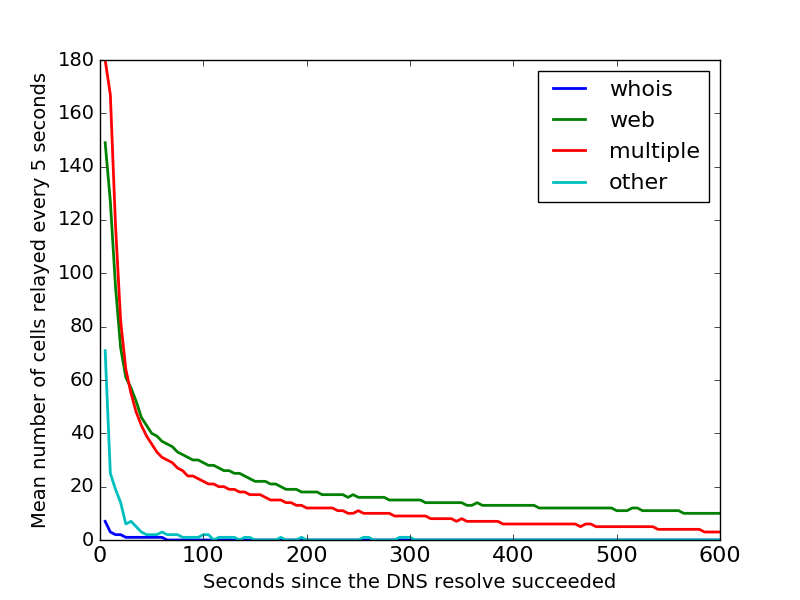
\includegraphics[width=0.4\textwidth]{images/exitmeasurement.png}
  \caption{Time Profile --- Average distribution of traffic across circuit
    lifetime beginning with the first DNS request.}
  \label{fig:statsa}
\end{figure}
\begin{figure} \centering
  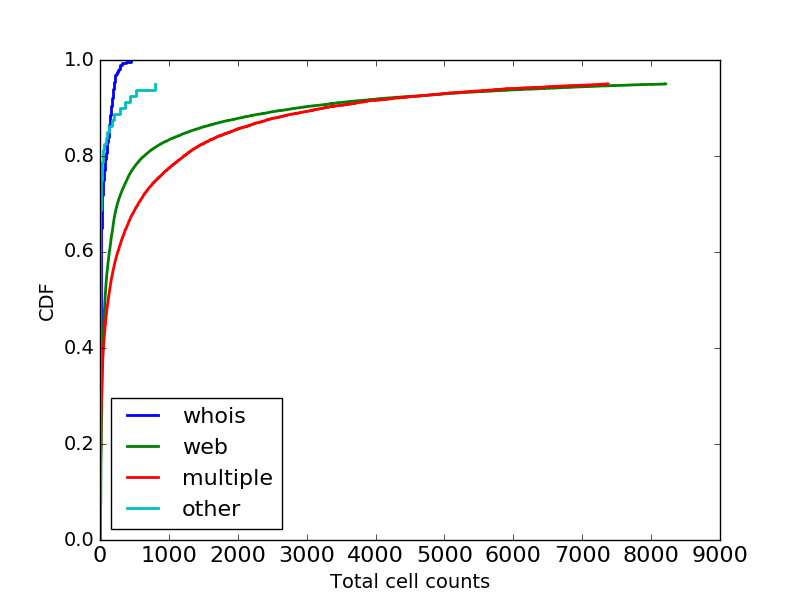
\includegraphics[width=0.4\textwidth]{images/totcellcountscdf.png}
  \caption{Total Counts --- Distribution of circuit size with respect to the
    total number of cells processed}
\label{fig:statsb}
\end{figure}


Our measurements successfully captured several important pieces of information
for the design and justification of moneTor. For example, one important task is
to determine the number of potential users that could benefit from paid
traffic. From Figure~\ref{fig:statsb}, we observe that $\approx 82\%$ of
circuits carrying only web traffic exchanged less than 1000 cells. While we
cannot deduce any statements about users, we can speak to the fraction of
circuits that may benefit from a payment channel in the Tor network, since
around $50\%$ of them do not carry data and less than $17\%$ of them carry at
least one web page. The remaining $18\%$ would appear to be better candidates
for moneTor.

It is also evident from Figure~\ref{fig:statsa} that most of the traffic is usually
carried within the first few tens of seconds, and that all types of traffic we
collected seems to follow the same rule. From that result, we believe that the
reliability of payment is critical within the first few seconds, especially from
a relay viewpoint. Our payment channels should ideally be established and ready
before the user begins to use the circuit. While this result cannot be
guaranteed for an unbounded number of circuits, a well-designed preemptive
circuit build strategy should do a sufficient job of eliminating channel
setup/establish latency in the average case.

%% In another area of research, it may be interesting to point out that since %
%$\approx 50\%$ of users do not carry data after their DNS request, some %
%adversary doing end-to-end correlation may prefer to use active attacks over %
%passive correlation to capture more identities.

\section{Simulated Validation}
\label{sec:experimentations}

Having established the empirical context for a channel payment scheme, we
validated our technical design via experiments performed on a prototype
software implementation within the native Tor codebase.

\subsection{Prototype}

A substantial contribution of the research is embedded within our implementation
of the moneTor framework. The modifications, applied to Tor release version
0.3.2.10, cover approximately fifteen thousand added lines of code across Tor's
core C software. We emphasize that the implementation is not a fully functional
prototype and is optimized solely for our experiments. Most notably, we
simulated crytographic operations in the nanopayment creation and close
procedures using CPU delays. These delays were tuned to conservatively reflect
real measurements in background work~\cite{green2017bolt}.\footnote{Extracted
  values are conservative in the sense that our zero-knowledge proofs require
  proving only a subset of the statements required in each corresponding Bolt
  zero-knowledge proof.} The partial prototype serves the following purposes in
our study.

\begin{enumerate}
\item An implementation covering nuances not explicitly
  covered in the protocol designs. In effect, we would like to show that there
  are no unexpected and prohibitive practical conflicts with the existing Tor
  design.
\item A platform to study the feasibility of premium circuit
  prioritization from a networking perspective.
\item A platform to obtain a rough factor-of-two approximation for all
  bandwidth, computation, and memory requirements of the system, both globally
  and at individual nodes.
\end{enumerate}

The first design purpose is clearly qualitative and we briefly note that we did
not discover any insurmountable logical flaws in the design. To analyze the
networking dynamics and resource consumption, we studied our implementations
through the following proceeding experiments.

\subsection{Methodology}
\label{subsec:methodology}

Experiments were conducted using the Tor shadow simulator
tool~\cite{jansen2011shadow}. We ran two sets of experiments at different
scales from a consensus document published in early February 2018. The first set featured 100 relays, 1000 clients, 10 intermediaries, and
ran for a total of 90 minutes. These experiments were used to gather information
concerning the system overhead and protocol execution times. The second set
featured 250 relays, 2500 clients, 25 intermediaries, 80 minutes of total run
time, and was used to measure the performance benefits conferred to premium
clients. In both cases, simulated traffic features 16\% \emph{bulk} clients who
continuously download 5 MiB files and 84\% \emph{web} clients who periodically
download 2 MiB files,\footnote{While 5 MiB bulk files are a common standard in
  Tor benchmarking~\cite{portal2018tormetrics}, 2 MiB web files reflect the
  approximate size of modern web pages~\cite{team2018httparchive}}. The number
and behavior of clients were chosen to satisfy (A) realistic congestion rates
measured by a transfer timeout percentage around 4\%~\cite{portal2018tormetrics}
and a historical bulk/web global traffic ratio of about
50\%~\cite{chaabane2010digging, mccoy2008shining}. Importantly, it should be
noted that neither the scale of our experiments nor the precise configuration of
client nodes are intended to be precise replicas of real-world conditions. Tor
networking is itself a complex area of research and we are content to adopt the
simplest model that will highlight the relatively crude networking needs of our
incentivization scheme.

\subsection{Experiments}
\label{subsec:experiments}
Our experiments are separated into three groups each capturing a separate
characteristic of the scheme.

\subsubsection{Global Overhead}

First, we attempt to show the total cost the moneTor scheme in terms of total
network throughput. To highlight worst-case performance, we configured a medium
scale experiment consisting of 100\% of premium clients and compare to a
baseline trial with 0\% premium clients. No actual traffic priority is
conferred. Since our algorithms makes use of some concurrent crytpographic
operations, we are concerned with the number of CPU cores available to most
relays. This information is not publicly available. As a result, we 
provide two trials with moneTor: one where we assume all nodes are running on
multi-core hardware and one in which all nodes are running on single-core
hardware. The results are summarized in Figure~\ref{fig:overhead}.

% Add information about how we simulate singlecore and multicore hardware
% That gonna overflow 12 pages, though :/

\begin{figure*} \centering
	\begin{subfigure}[t]{0.32\textwidth} \centering
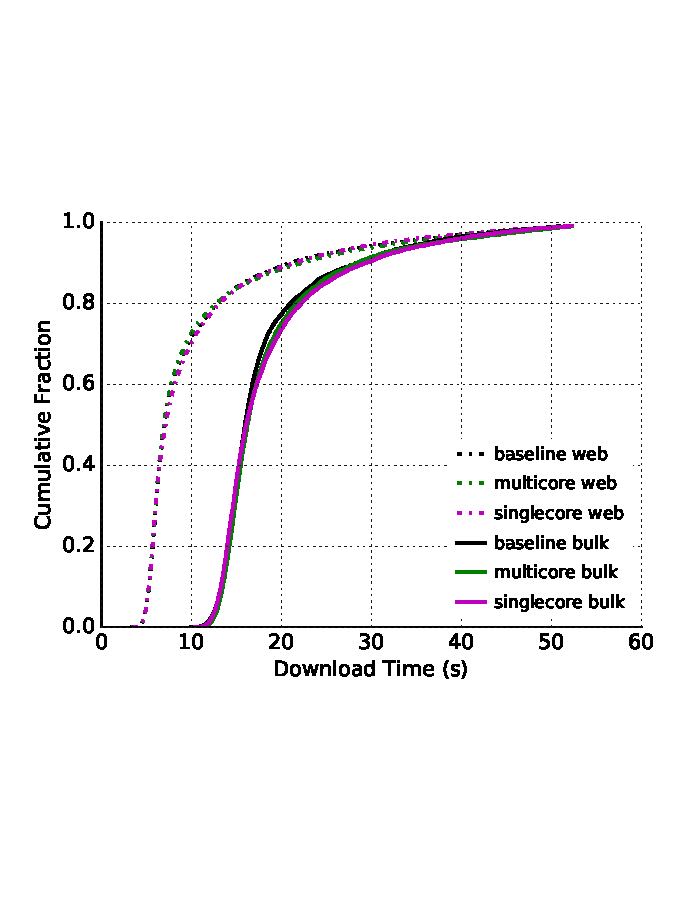
\includegraphics[trim={0 3cm 0 3cm}, clip, width=1.0\textwidth]{images/overhead_downloadtime.pdf}
		\caption{Download Time Overhead}
		\label{fig:overhead_ttlastbyte}
	\end{subfigure}
	\begin{subfigure}[t]{0.32\textwidth} \centering
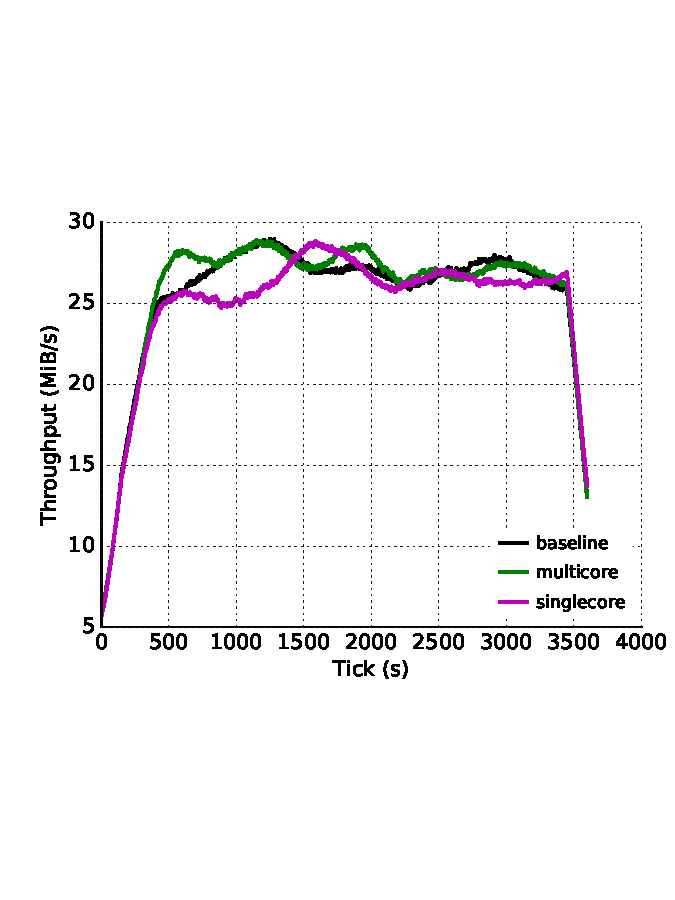
\includegraphics[trim={0 3cm 0 3cm}, clip, width=1.0\textwidth]{images/overhead_throughput.pdf}
		\caption{Throughput Overhead}
		\label{fig:overhead_throughput}
	\end{subfigure}
	\begin{subfigure}[t]{0.32\textwidth} \centering
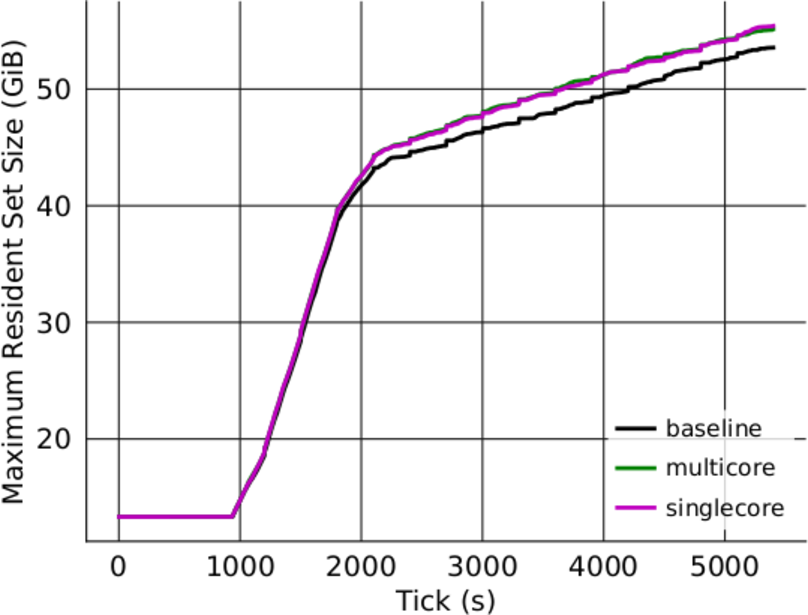
\includegraphics[trim={0 3cm 0 3cm}, clip, width=1.0\textwidth]{images/overhead_memory.pdf}
		\caption{Simulation Memory}
		\label{fig:overhead_shadow}
	\end{subfigure}
	\caption{Global Overhead --- Comparison of overhead in pure multicore
          and singlecore network
          conditions. Figure~\ref{fig:overhead_ttlastbyte} shows two sets of
          download time CDF curves for each file size (2 MiB and 5 MiB),
          Figure~\ref{fig:overhead_throughput} shoes the 5 minute moving average
          throughput over time, and Figure~\ref{fig:overhead_shadow} shows the
          memory consumption across the experiment lifetime. The simulation
          includes 100 relays, 2 authorities, 1 ledger authority, 10
          intermediaries and 1000 Tor clients scaled down from the public
          consensus file `2018-02-03-00-00-00-consensus'.}
	\label{fig:overhead}
\end{figure*}

Our findings indicate that even in the worst case scenario, our system incurs
statistically negligible overhead at these scales across all three measures of
download time, throughput, and memory usage. This in line with the raw bandwidth
overhead observations in which a small fraction ($< 1\%$) of the network traffic
is attributable to moneTor payment messages. This is true for all of our trials
which feature a payment rate of 1 payment (1 cell) every 1000 data cells
exchanged in either direction. It is also possible to increase the payment rate
for more fairness if needed, as long as the total overhead induced from control
cells is kept under an acceptable fraction of the overall data bandwidth. 
%%%
% Reading this sentence appears to be unclear to me
%%%
%This
%low overhead cost is separate from adverse networking effects of prioritization,
%which has the potential to more drastically affect performance.

%\begin{table}
%  \caption[Overhead Throughput Total]{\textbf{Overhead Throughput Total} Total
%    transferred application traffic over the duration of the over head trials
%    compared to total transferred payment traffic.}
%  \begin{center}
%    \begin{tabular}{ c c c }
%      & Throughput (GiB) & Payment Traffic (GiB) \\ \hline
%      Baseline & 128.4 & 0.000 \\
%      Multi-Core & 129.1 & 0.449 \\
%      Single-Core & 127.6 & 0.396
%    \end{tabular}
%  \end{center}
%  \label{tab:overhead}
%\end{table}

\subsubsection{Payment Latency}

Given results from our data collection, we surmise that payment latency is a
crucial factor in servicing our front-loaded clients. To this end, we measure
the distribution of completion times for various steps in the protocol. The
results shown here are collected from a worst case multicore experiment
featuring 100 relays and 1000 clients all of whom run premium circuits. To
highlight the effects of native latency in the Tor network, we show payments
split across each relay role of guard, middle, and exit. Recall that moneTor
makes use of high-overhead, low-marginal cost payment channels. The bulk of the
cost in our scheme lies in the conduction of the nanopayment channel
\emph{establish} and \emph{close} protocols as shown in
Figure~\ref{fig:payments_establish} and Figure~\ref{fig:payments_close}. Notice
that close operations are about twice as time consuming as establish operations
reflecting the need for the relay to close his half of the nanopayment channel
before the client can complete hers. Figure~\ref{fig:ttfp} illustrates time to
first payment, our most revealing latency metric. This measure includes the
overhead in channel establishment when we do not have available preemptive
channels. In the best case scenario, when all three payment channels have been
correctly pre-built for the circuit, this measure is equivalent to a single trip
toward each relay. Comparing this Figure~\ref{fig:ttfp} to
Figure~\ref{fig:payments_establish}, we observe the effectiveness of preemptive
channel building.

\begin{figure*} \centering
	\begin{subfigure}[t]{0.32\textwidth} \centering
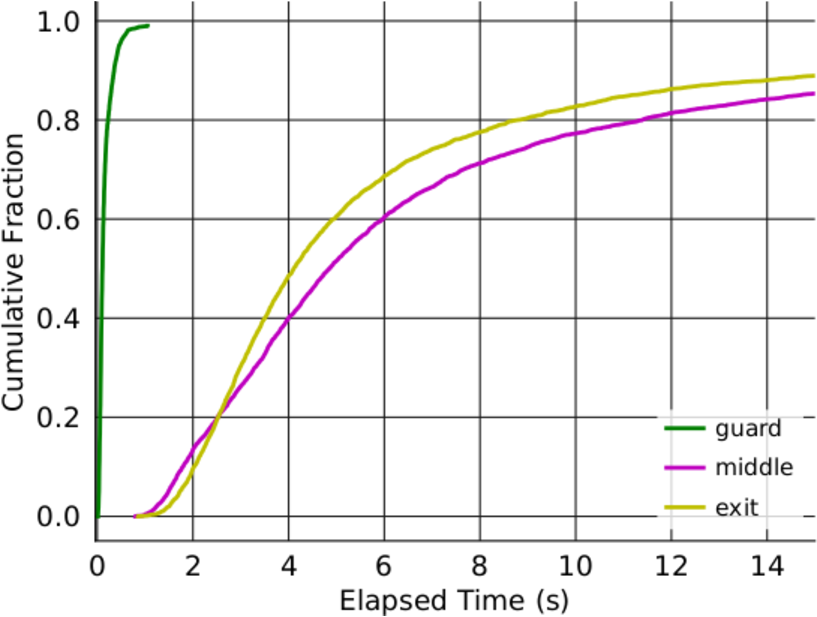
\includegraphics[trim={0 3cm 0 3cm}, clip, width=1.0\textwidth]{images/payment_establish.pdf}
		\caption{Nano-Establish}
\label{fig:payments_establish}
	\end{subfigure}
	\begin{subfigure}[t]{0.32\textwidth} \centering
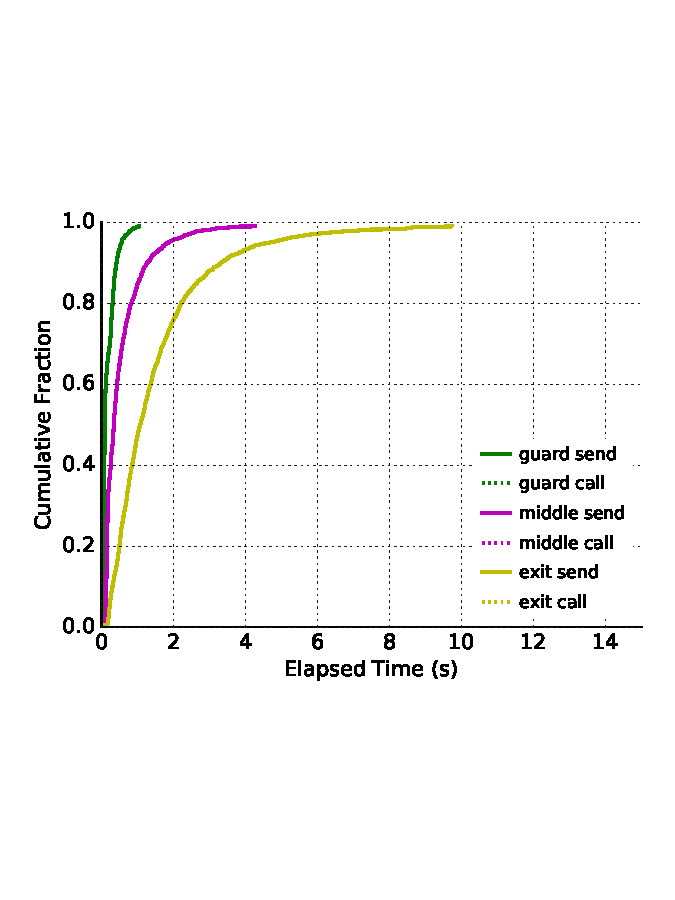
\includegraphics[trim={0 3cm 0 3cm}, clip, width=1.0\textwidth]{images/payment_pay.pdf}
		\caption{First Payment}
\label{fig:ttfp}
	\end{subfigure}
	\begin{subfigure}[t]{0.32\textwidth} \centering
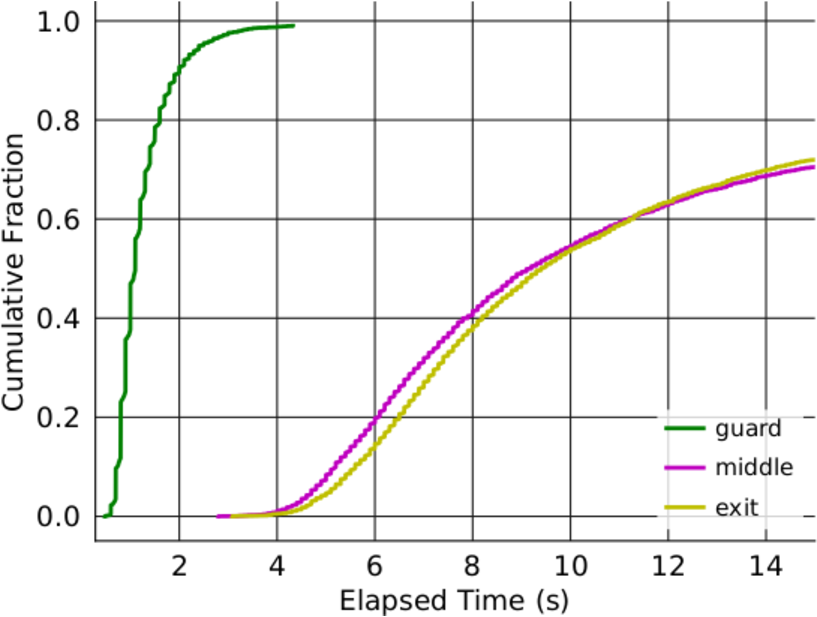
\includegraphics[trim={0 3cm 0 3cm}, clip, width=1.0\textwidth]{images/payment_close.pdf}
		\caption{Nano-Close}
\label{fig:payments_close}
	\end{subfigure}
	\caption{Protocol Execution Time --- Time to finish each protocol step
          split across interactions with each of the three relay. The simulation
          includes 100 relays, 2 authorities, 1 ledger authority, 10
          intermediaries and 1000 Tor clients scaled down from the public
          consensus file `2018-02-03-00-00-00-consensus'.}
\label{fig:latencymeasurements}
\end{figure*}

In all protocol phases, we observe that latency for guard relays are negligible
in comparison to the middle and exit relays, further validating our design
decision to implement special directly paid guard channels.

\subsubsection{Network Priority}
\label{sec:priority_exp}

Our final set of experiments studies the success of our scheme in delivering
prioritized traffic for premium users. To perform this analysis, we prepared
sets of three small experiments with varying modifier priorities
$\alpha \in \{0, 0.25, 0.5\}$, where $\alpha = 0$ represents the baseline
control. Our first set of experiments assuming 50\% of premium users is shown in
Figures \ref{fig:modifier_pr50_web}, \ref{fig:modifier_pr50_bulk}, and
\ref{fig:modifier_pr50_all}. From this illustration, is it evident that premium
users enjoy an advantage in internet speed compared to nonpremium users and that
this advantage is more pronounced with the higher priority modifier. Moreover,
the evenly split premium and nonpremium performance ``averages out'' to
approximately mirror the baseline experiment, indicating little loss in overall
network performance, and confirming our overhead experiment.

A more realistic model should most likely assume a smaller minority of premium
users. We therefore conducted a separate set of experiments to study an
environment comprised of only 25\% premium users who, according to
Equation~\ref{eq:flow}, should expect an even greater benefit on a per-user
basis. Figures \ref{fig:modifier_pr25_web}, \ref{fig:modifier_pr25_bulk}, and
\ref{fig:modifier_pr25_all} shows that this is indeed the result. Users across
the spectrum of web speed enjoyed $\approx 100\%$ improvements in download
speeds relative to nonpremium users --- likely enough to induce some amount of
monetary exchange. 


\begin{figure*} \centering
	\begin{subfigure}[t]{0.32\textwidth} \centering
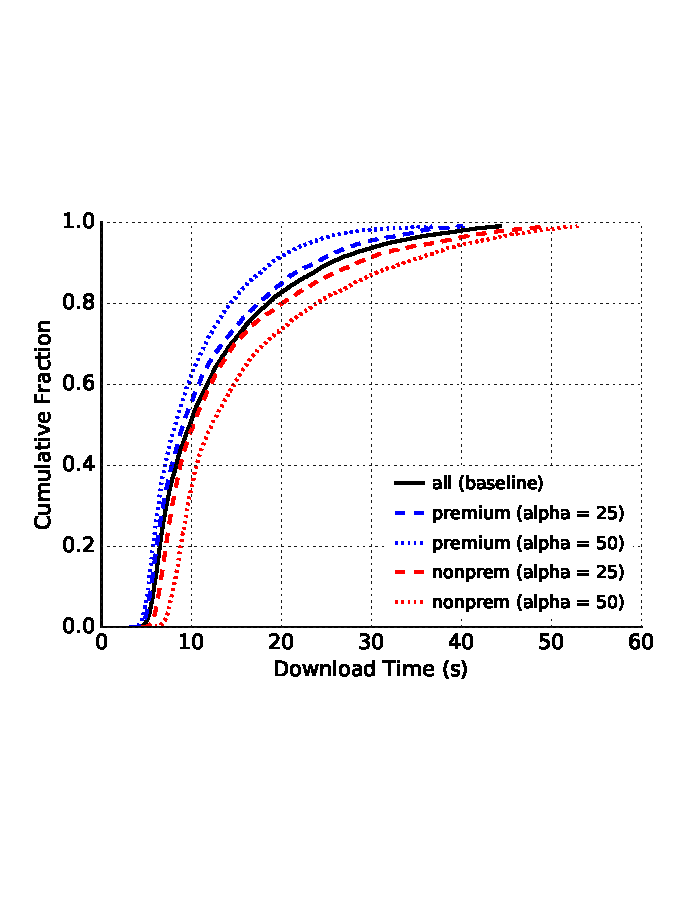
\includegraphics[trim={0 3cm 0 3cm}, clip, width=1.0\textwidth]{images/modifier_pr50_web.pdf}
		\caption{Web Download Time}
\label{fig:modifier_pr50_web}
	\end{subfigure}
	\begin{subfigure}[t]{0.32\textwidth} \centering
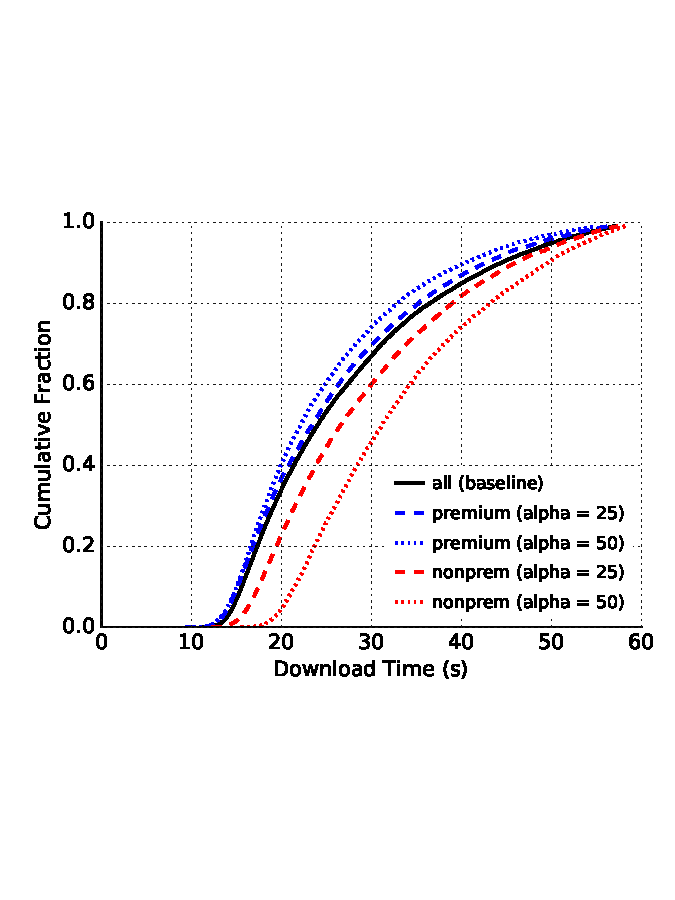
\includegraphics[trim={0 3cm 0 3cm}, clip, width=1.0\textwidth]{images/modifier_pr50_bulk.pdf}
		\caption{Bulk Download Time}
\label{fig:modifier_pr50_bulk}
	\end{subfigure}
	\begin{subfigure}[t]{0.32\textwidth} \centering
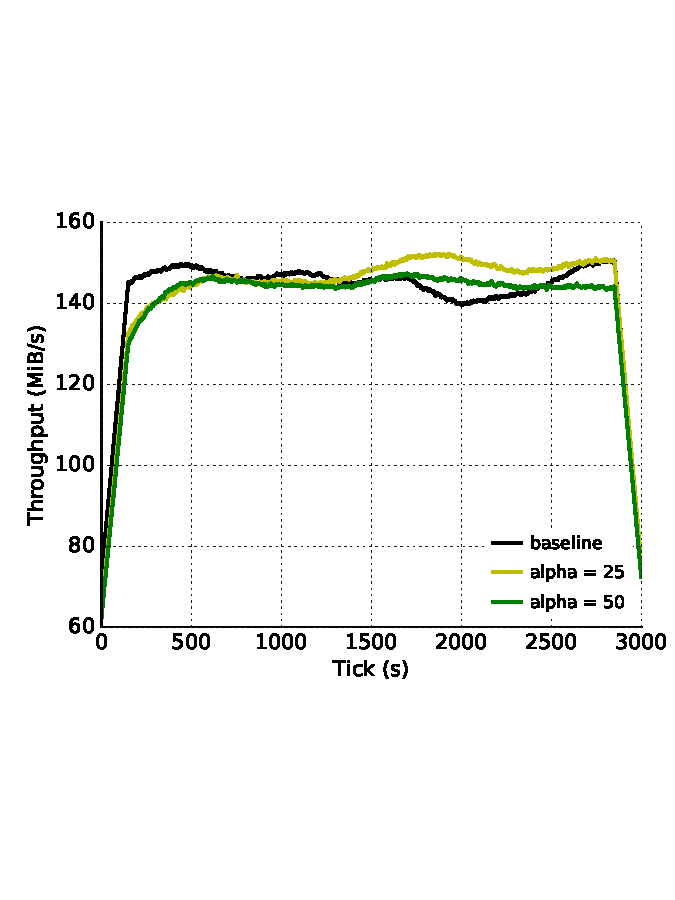
\includegraphics[trim={0 3cm 0 3cm}, clip, width=1.0\textwidth]{images/modifier_pr50_all.pdf}
		\caption{Throughput}
\label{fig:modifier_pr50_all}
	\end{subfigure}
	\begin{subfigure}[t]{0.32\textwidth} \centering
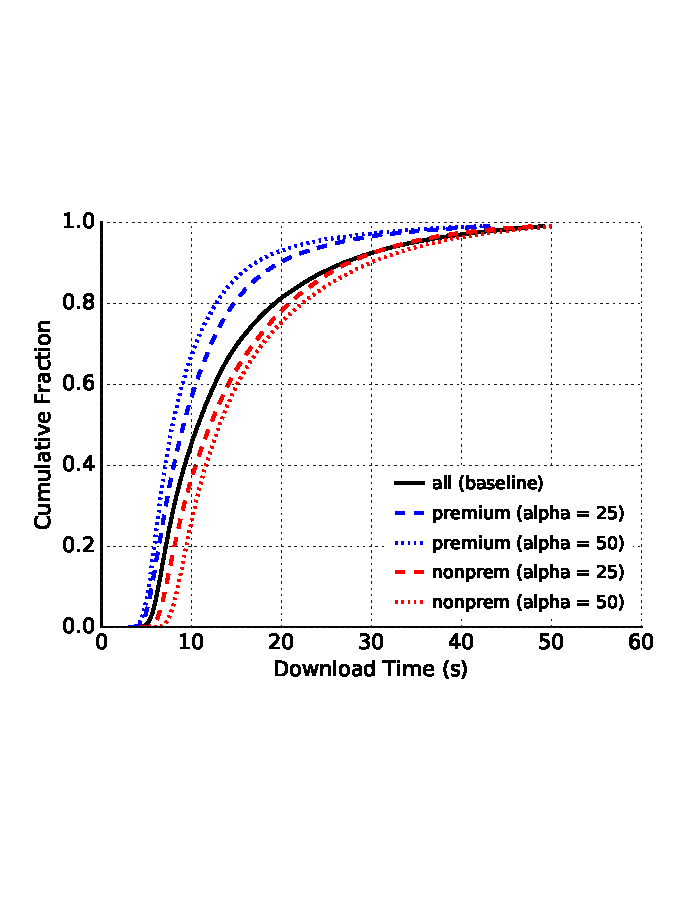
\includegraphics[trim={0 3cm 0 3cm}, clip, width=1.0\textwidth]{images/modifier_pr25_web.pdf}
		\caption{Web Download Time}
\label{fig:modifier_pr25_web}
	\end{subfigure}
	\begin{subfigure}[t]{0.32\textwidth} \centering
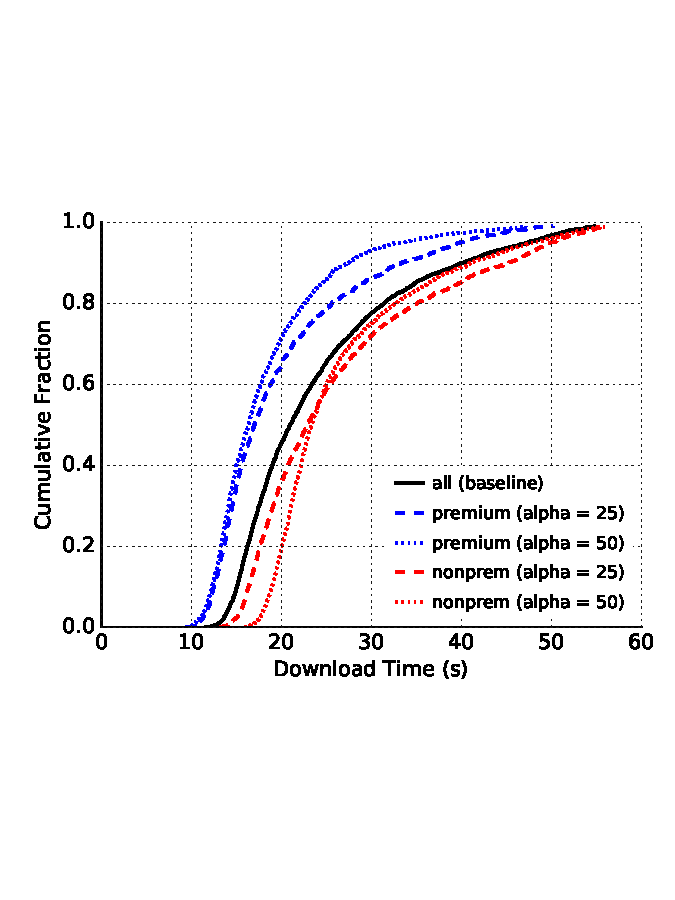
\includegraphics[trim={0 3cm 0 3cm}, clip, width=1.0\textwidth]{images/modifier_pr25_bulk.pdf}
		\caption{Bulk Download Time}
\label{fig:modifier_pr25_bulk}
	\end{subfigure}
	\begin{subfigure}[t]{0.32\textwidth} \centering
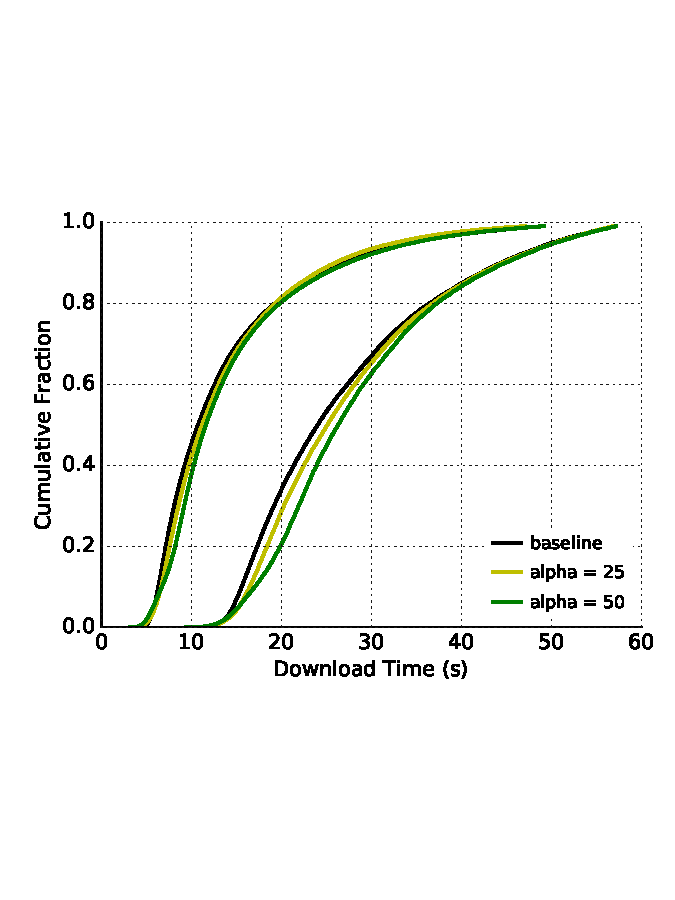
\includegraphics[trim={0 3cm 0 3cm}, clip, width=1.0\textwidth]{images/modifier_pr25_all.pdf}
		\caption{Throughput}
\label{fig:modifier_pr25_all}
	\end{subfigure}
	\caption{Prioritization Benefit --- Performance differentiation between
          paid and unpaid users. The first row displays results with 50\%
          premium users while the second row displays results for 25\% premium
          users. Simulations feature 250 relays, 2 authorities, 1 ledger
          authority, 25 intermediaries and 2500 Tor clients scaled down from the
          public consensus file `2018-02-03-00-00-00-consensus'.}
\label{fig:modifier}
\end{figure*}

%\begin{table}
%  \caption[Prioritized Throughput]{\textbf{Prioritized Throughput} Tabulate total
%    number of successful file transfers and timeout errors across varying levels
%    of prioritization}
%  \begin{center}
%    \begin{tabular}{ c c c c}
%      & Throughput & Timeouts & Timeout \\
%      & (GiB) & (Web) & (Bulk) \\ \hline
%      $\alpha = 0.00$ & 427 & 115 & 354 \\ \hline
%      $\alpha = 0.25,\ pr\% = 50$ & 429 & 206 & 404 \\
%      $\alpha = 0.25,\ pr\% = 25$ & 433 & 231 & 459 \\ \hline
%      $\alpha = 0.50,\ pr\% = 50$ & 420 & 233 & 356 \\
%      $\alpha = 0.50,\ pr\% = 25$ & 414 & 381 & 513 \\
%    \end{tabular}
%  \end{center}
%  \label{tab:modifier}
%\end{table}

%%% Local Variables:
%%% mode: latex
%%% TeX-master: "../main"
%%% End:


\section{Limitations}
\label{sec:limitations}

\section{Code and Data Reproducibility}
\label{sec:code}

\section{Conclusion}
\label{sec:conclusion}
\bibliographystyle{ACM-Reference-Format}
\bibliography{ccs-sample}
\end{document}
